\documentclass[12pt,letterpaper]{article}
\usepackage[T1]{fontenc}
\usepackage[sfdefault,scaled=.9]{FiraSans}
\usepackage{newtxsf}
\usepackage[tmargin=1in,bmargin=1in,lmargin=1in,rmargin=1in]{geometry}
\usepackage[dvipsnames]{xcolor}
\usepackage{tikz}
\usepackage{array}
\usepackage{graphicx}
\usepackage{caption}
\usepackage{subcaption}
\usepackage{pifont}
\usepackage{empheq}
\usepackage{cancel}
\usepackage{amsmath,mathtools}
\usepackage{amssymb}
\usepackage{amsfonts}
\numberwithin{equation}{section}
\usepackage{bm}
\usepackage[breaklinks=true,colorlinks=true,linkcolor=purple,urlcolor=purple,citecolor=blue,%
  pdftitle={Detroit Blight Ticket Compliance},
  pdfsubject={cs.LG},%
  pdfauthor={Cedric Yu}]{hyperref}
%\usepackage{filecontents}
\usepackage{dsfont}
\usepackage{soul}
\usepackage{slashed}
\usepackage{pbox}
\usepackage{float}
\usepackage[nottoc,notlot,notlof]{tocbibind}
\allowdisplaybreaks
\hbadness=10000
\hfuzz=\maxdimen
\setcounter{tocdepth}{2}
\hypersetup{pdfpagemode=UseNone}
\usepackage{listings}

\DeclarePairedDelimiter\ceil{\lceil}{\rceil}
\DeclarePairedDelimiter\floor{\lfloor}{\rfloor}

\usepackage[most]{tcolorbox}
\tcbset{myformula/.style={colback=white, %yellow!10!white,
    colframe=black, %red!50!black,
    top=5pt,bottom=5pt,left=5pt,right=5pt,
    toprule=0.5pt,bottomrule=0.5pt,leftrule=0.5pt,rightrule=0.5pt,
    boxsep=0pt,
    arc=0pt,
    outer arc=0pt,
}}

%Symbols for author emails
 \makeatletter
\def\@fnsymbol#1{\ensuremath{\ifcase#1 \or \natural\or \flat\or \sharp\or
   \quarternote\or \halfnote\or \twonotes\or \eighthnote \or \dagger\dagger
   \or \ddagger\ddagger \else\@ctrerr\fi}}
    \makeatother

\begin{document}
\renewcommand{\Im}{{\rm Im}\,}
\renewcommand{\Re}{{\rm Re}\,}
\newcommand{\diag}{{\rm diag} \, }
\newcommand{\Tr}{{\rm Tr}\,}
\newcommand{\tr}{{\rm tr}\,}
\newcommand{\C}{{\mathcal{C}}}

\title{\vspace{-2.5cm}\color{PineGreen}\textbf{Detroit Blight Ticket Compliance}}
\date{} % remove date
\author{Cedric Yu\footnote{\href{mailto:cedric.yu@nyu.edu}{cedric.yu@nyu.edu}. Last updated: \today.}}
% \email{cedric.yu@nyu.edu}
%\affiliation{%
%Department of Physics, New York University New York, NY
%}%
\maketitle
\vspace{-1cm}
\begin{abstract}
We summarise our findings on the (expired) \href{https://www.kaggle.com/c/detroit-blight-ticket-compliance/overview}{Kaggle competition}--- which was also the final assignment of the ``Applied Machine Learning in Python" course on \href{https://www.coursera.org/learn/python-machine-learning}{Coursera} offered by The University of Michigan--- predicting whether a given blight ticket in Detroit will be paid on time. This report was written as I revisited this project after submitting the assignment. This time I did things differently from the last time.
\end{abstract}

%Table of contents
%\begingroup
%\hypersetup{linkcolor=black}
%\hrule height 0.75pt
%\tableofcontents
%\vspace{0.8cm}
%\hrule height 0.75pt
%\endgroup

%**\vphantom{}
%\begin{align}
% A &=     \left(\int XXX       \right.\nonumber\\
%   &\qquad \left.\vphantom{\int} YYY \dots \right)
%\end{align}

%**Box for align
%\begin{empheq}[box=\fbox]{align}
%ABD & DEF\\
%&=GHI
%\end{empheq}

%Inner box with empheq for align
%\begin{empheq}[innerbox=\fbox,
%left=L\Rightarrow]{align}
%a&=b\\
%E&=mc^2 + \int_a^a x\, dx
%\end{empheq}

%**Box for align using tcolorbox; box includes equation number
%\begin{tcolorbox}[ams align,myformula]
%ABD & DEF\\
%&=GHI
%\end{tcolorbox}

%**left brace for subequations; (1.1a) and (1.1b)
%\begin{subequations}
%\begin{empheq}[left=\empheqlbrace]{align}
%s&=1\\
%o&=8
%\end{empheq}
%\end{subequations}


%**Move left the whole align with long formulas. \hspace*{-2cm}\vbox{  \begin{align} ... \end{align}}
%\hspace*{-2cm}\vbox{
%\begin{align}
%R_1(z)&\rightarrow (1-z)^{\frac{\Delta}{2}}\left(1+\mathcal{O}(1-z)\right)\frac{\Gamma(1-ik_T)\Gamma(1-\Delta)}{\Gamma(1-\frac{\Delta}{2}-ik_{\bar{w}})\Gamma(1-\frac{\Delta}{2}-ik_w)}\nonumber\\
%&\qquad\qquad+(1-z)^{\frac{2-\Delta}{2}}\left(1+\mathcal{O}(1-z)\right)\frac{\Gamma(1-ik_T)\Gamma(\Delta-1)}{\Gamma(\frac{\Delta}{2}-ik_{\bar{w}})\Gamma(\frac{\Delta}{2}-ik_w)}\\
%R_2(z)&\rightarrow (1-z)^{\frac{\Delta}{2}}\frac{\Gamma(1+ik_T)\Gamma(1-\Delta)}{\Gamma(1-\frac{\Delta}{2}+ik_{\bar{w}})\Gamma(1-\frac{\Delta}{2}+ik_w)}+(1-z)^{\frac{2-\Delta}{2}}\frac{\Gamma(1+ik_T)\Gamma(\Delta-1)}{\Gamma(\frac{\Delta}{2}+ik_{\bar{w}})\Gamma(\frac{\Delta}{2}+ik_w)}.
%\end{align}}

%** multiple lines in one equation number
%\begin{equation}
%\begin{aligned}
%I&JKL\\
%&=MN
%\end{aligned}
%\end{equation}

%** splits formulas in align
%\begin{align}
%\begin{split}
%Rs&dd\\
%&+ss
%\end{split}
%\\
%\begin{split}
%aa&dd\\
%&+ff
%\end{split}
%\end{align}

%**  trim={<left> <lower> <right> <upper>}. clip activates cropping.
%\begin{figure}[h]
%\begin{center}
%\includegraphics[trim={0 390 400 0},clip,width=0.68\linewidth,keepaspectratio]{ADM_fig.pdf}
%\caption{Wald Fig. 10.2. The shift vector $N^a$ and the lapse function $N$.}
%\end{center}
%\end{figure}

%\begin{figure}[H]
%\centering
%\begin{subfigure}{0.8\textwidth}
%  \centering
%  \includegraphics[width=.8\linewidth,keepaspectratio]{Torus_two_tubes.pdf}
%\caption{The solid.}\label{Torus_two_tubes}
%\end{subfigure}%
%\linebreak
%\begin{subfigure}{.8\textwidth}
%  \centering
%  \includegraphics[width=.8\linewidth,keepaspectratio]{torus_dome.pdf}
%  \caption{The sad.}
%  \label{torus_dome}
%\end{subfigure}
%\caption{The sss.}
%\label{Torus_two_tubes0}
%\end{figure}

%\det\nolimits^{\perp}{(\nabla^2+2-m^2)}

%\hyperref[abc]{Section \ref*{abc}}

%\section{\texorpdfstring{$AdS_3$}{AdS3} Notation}

\section{Problem Statement}
In this competition, we are tasked with predicting whether a given set of blight tickets will be paid on time. Blight violations are issued by the city of Detroit, Michigan, to individuals who allow their properties to remain in a deteriorated condition. Every year, the city issues millions of dollars in fines to residents and every year, but many of these fines remain unpaid. Enforcing unpaid blight fines is a costly and tedious process, so the city wants to know how to increase blight ticket compliance.

\subsection{Datasets}
We are given the training and test datasets. There are too many given features to be listed here; see the description in the accompanying \verb|.py| files. The features include the violator's name and mailing address, address of the property in violation, violation code, ticket issue datetime, hearing datetime and details of the fine. There are also features that are only available in the training set but not in the test set; we discard those features.

The target is \verb|compliance|: \verb|1| means responsible and compliant, \verb|0| means responsible but non-compliant, and  \verb|NaN| means not responsible.

\subsection{Evaluation Metric}

The results will be evaluated by the area-under-the-curve (auc) of the Receiver operating characteristic (ROC) curve; we want to maximise auc, so that we can maximise the true positive rate and minimise the false positive rate by adjusting the decision threshold by which we classify an instance into \verb|0| or \verb|1|.

\subsubsection*{Preliminary Observations and Processing}
The training set (\verb|train.csv|) contains $250,306$ instances, while the test set (\verb|test.csv|) has $61,001$ instances. 

We first parse the datetime columns, namely \verb|ticket_issued_date| and \verb|hearing_date|, of both the training and test sets, extract the respective \verb|year|, \verb|month|, \verb|day|, \verb|weekday| and \verb|hour| features, and save the sets as new \verb|csv| files. The datasets do not take up a large amount of memory, so we do not downcast the data types of the columns.

An immediate observation is that, in the training set there are $90,426$ instances with target label \verb|NaN| which means ``not responsible". Obviously, the first we do is to drop these instances, after which we are left with $159,880$ instances. Next, we drop the columns \verb|payment_amount|, \verb|payment_date|, \verb|payment_status|, \verb|balance_due|, \verb|collection_status|, and \verb|compliance_detail| which are only available in the training set. After that, we have several columns with some number of missing values: 
\begin{lstlisting}[language=Python, basicstyle=\footnotesize]
violator_name                     26
violation_zip_code            159880
mailing_address_str_number      2558
mailing_address_str_name           3
state                             84
zip_code                           1
non_us_str_code               159877
grafitti_status               159880
hearing_date_year                227
hearing_date_month               227
hearing_date_weekday             227
hearing_date_day                 227
hearing_date_hour                227
\end{lstlisting}
Of these, \verb|violation_zip_code|, \verb|non_us_str_code| and \verb|grafitti_status| have so many missing values that we expect to drop them.

\section{Exploratory Data Analysis}

We make plots in \verb|dataset_study.py|.

\subsection{Target: \texttt{compliance}}


\vspace*{-12pt}

\begin{figure}[H]
\begin{center}
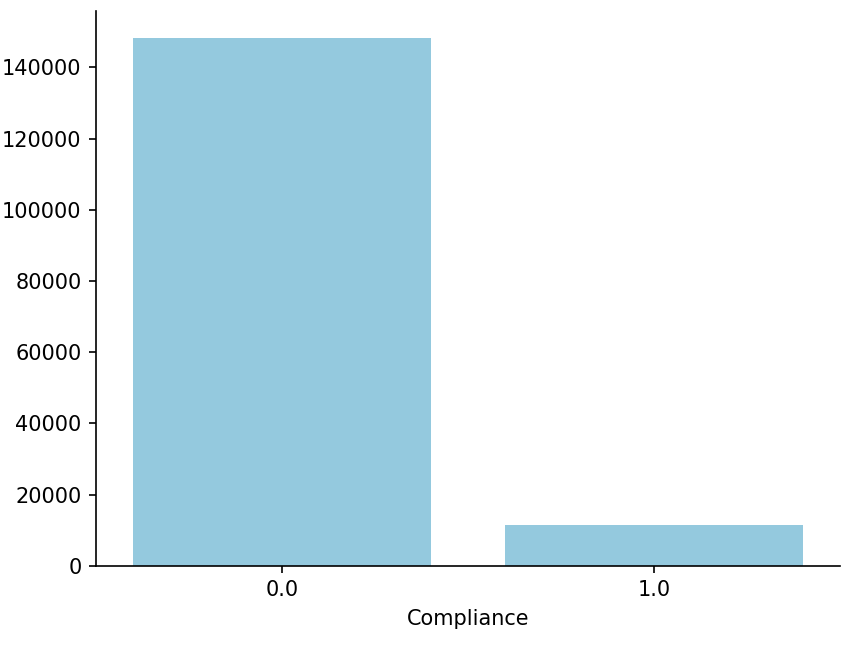
\includegraphics[width=0.6\linewidth,keepaspectratio]{plots/train_compliance.png}
\caption{\texttt{compliance} in the training set.}\label{compliance}
\end{center}
\end{figure}

Having discarded the instances with \verb|compliance| being \verb|NaN| meaning not responsible, from the training set, we first get \hyperref[compliance]{Figure \ref*{compliance}} for the target label.

That is, the vast majority of the tickets were not complied; that's why we have a problem to solve to begin with. This means we have a \textbf{class imbalance}. This needs to be taken care of when we train machine learning models.

\subsection{Datetime Features}

Next, we look at the datetime features extracted from the features \verb|ticket_issued_date| and \verb|hearing_date|. We learn that the ticket issue dates in the training set were from the years 1988, 2004-2011, while those in the test set were from the years 2012-2016. There are respectively only 1 and 15 instances in years 1988 and 2004. This motivates us to drop instances in years 1988 and 2004. Including dropping the \verb|NaN| in \verb|compliance|, this makes \textbf{two truncations}. Similarly, from \verb|hearing_date| we learn that the hearings in the test set happened after those in the training set. Anticipating the use of tree-based algorithms, the \verb|year| features will be less than useful; we drop these two columns. The are missing values in \verb|hearing_date|; we will fill those with the most frequent occurrence.

Next, for the \verb|month|, \verb|day|, \verb|weekday| and \verb|hour| features, we do not see anything particular that stands out, except that hearings only took place on weekdays (as expected). Another thing to look at is how we should encode these categorical features. We looked at the frequency plots and the target mean plots to draw inspirations, but did not always see any particular preference towards one or another. See e.g. \hyperref[month]{Figure \ref*{month}} for \verb|ticket_issued_date_month|.


\begin{figure}[H]
\centering
\begin{subfigure}{0.6\textwidth}
  \centering
  \includegraphics[width=1.\linewidth,keepaspectratio]{plots/1_datetime/ticket_month_training.png}
\caption{Count plot}
\end{subfigure}% 
\hspace*{-2cm}
\begin{subfigure}{.6\textwidth}
  \centering
  \includegraphics[width=1.\linewidth,keepaspectratio]{plots/1_datetime/ticket_month_mean_compl_training.png}
  \caption{Target mean}
\end{subfigure}
\caption{Histograms for \texttt{ticket\_issued\_date\_month} from the twice-truncated training set.}
\label{month}
\end{figure}

\subsection{Mailing Address Features}\label{address}

We now look at the features about the violators' mailing addresses. As a reminder, from the last section we saw too many \verb|NaN| for \verb|violation_zip_code|, so we dropped that column. Among the relevant columns, we only keep the columns \verb|country|, \verb|state|, \verb|city| and \verb|zip_code|, which should already contain enough information; we drop \verb|mailing_address_str_number|, \\\verb|mailing_address_str_name| and \verb|non_us_str_code|.

\verb|country| contains \verb|USA|, \verb|Cana|, \verb|Aust|, \verb|Egyp| and \verb|Germ|. Only 11 in the twice-truncated training set are not \verb|USA|. Looking at the \verb|state| feature of those with \verb|country == USA|, we find that it contains some non-US states(+DC), such as \verb|QC| and \verb|BC| in Canada. Our way of cleaning this up is as follows. We now use \verb|country| to classify whether a mailing address is a US address, or not. To count as \textit{really} being in the US, we demand that \verb|state| is one of the 50 states(+DC). 

Looking at \verb|state|, we find the most are \verb|MI| (obviously). As such, we will use frequency encoding on this feature.

Of those with mailing addresses inside the US, we study the \verb|zip_code|. Most are 5-digit as expected, but there are also some with less than 5 digits, which we count as invalid and set as \verb|'0'|. Most other ones are 9- or 10-digit, which are genuine zip codes with the extra 4-digit suffix, with or without a hyphen. We extract the 5-digit zip codes using \verb|regex|. There are respectively 113 and 2 instances with 6- and 7-digit \verb|zip_code|. A closer look at the mailing addresses suggests that those number are somewhat close but not exactly the correct zip codes. Nonetheless, they do not make up a large part of the dataset, so we simply just extract the first 5 digits as the zip codes. For the non-US instances, we set the zip codes to \verb|'0'|.


\subsection{\texttt{violation\_code} and \texttt{violation\_description}}

The \verb|violation_description| is just the explanation of the \verb|violation_code| in words; drop the former.

\subsection{Fine and Fees}

We find that \verb|admin_fee| and \verb|state_fee| are the same for all instances. \verb|clean_up_cost| is zero for all instances in the training set. Though the test set has $1,580$ instances out of $61,001$ with non-zero \verb|clean_up_cost|, We cannot tell anything about it from the training data, so we drop this too. \verb|judgment_amount| is a simple sum of fees.

All in all, we drop \verb|admin_fee|, \verb|state_fee|, \verb|clean_up_cost| and \verb|judgment_amount|.



\section{Feature Pre-processing and Engineering}

We now describe the feature pre-processing and engineering procedure, implemented in \\\verb|pre-processing.py|.

\subsection{Workflow}

We first describe our workflow, where the starting point is the datetime-processed training set.

\begin{enumerate}
\item Load datetime-processed training set containing \verb|year|, \verb|month|, \verb|weekday|, \verb|day|, \verb|hour| extracted from parsed datetime columns \verb|ticket_issued_date| and \verb|hearing_date|
\item Diacard columns that are not in the test set
\item Drop instances with \verb|NaN| target label \verb|compliance|
\item Restrict to instances with \verb|ticket_issued_date_year| after year 2004
\item Fill (the one) \verb|NaN| of \verb|zip_code| with \verb|'0'|
\item Separate features and labels
\item Train-validation split: we use a 80-20 split
\item Drop the following columns:
\begin{lstlisting}[language=Python, basicstyle=\footnotesize]
cols_to_drop1 = ['ticket_id', 'violation_zip_code', 
'violation_description', 'admin_fee', 'state_fee', 
'judgment_amount', 'inspector_name', 'violator_name', 
'violation_street_number', 'violation_street_name', 
'mailing_address_str_number', 'mailing_address_str_name', 
'non_us_str_code', 'city', 'clean_up_cost', 'grafitti_status', 
'ticket_issued_date_year', 'hearing_date_year']
\end{lstlisting}
\item Process mailing addresses
\item Fillna in \verb|hearing_date| columns with most frequent occurrences
\item Encode categorical variables
\item Fill any remaining missing values (due to encoding) by the columns means
\item Apply \verb|MinMaxScaler| (we will use KNN)
\item Repeat Steps 8-13 for the datetime-processed test set.
\end{enumerate}


\subsection{Processing Mailing Addresses}

To process the mailing address features in the way outlined in \hyperref[address]{Section \ref*{address}}, we use define the following function which is applied on the datasets:

\begin{lstlisting}[language=Python, basicstyle=\footnotesize]
import re

def country_zip_process(df) :
    
    US_states = ["AL", "AK", "AZ", "AR", "CA", "CO", "CT", "DC", "DE", "FL", "GA", 
              "HI", "ID", "IL", "IN", "IA", "KS", "KY", "LA", "ME", "MD", 
              "MA", "MI", "MN", "MS", "MO", "MT", "NE", "NV", "NH", "NJ", 
              "NM", "NY", "NC", "ND", "OH", "OK", "OR", "PA", "RI", "SC", 
              "SD", "TN", "TX", "UT", "VT", "VA", "WA", "WV", "WI", "WY"]
    
    def country_zip_func(row) : 
        if row['state'] in US_states: 
            row['country'] = 1
            if (len(re.findall("\d{5,5}",row['zip_code'])) > 0):
                row['zip_code']=int(re.findall("\d{5,5}",row['zip_code'])[0])
            else:
                row['zip_code'] = 0
        else : 
            row['country'] = 0
            row['state'] = 'not_in_US'
            row['zip_code'] = 0
        return row
    
    df1 = df.apply(country_zip_func, axis = 1)
    
    return df1
\end{lstlisting}

\subsection{Fillna in \texttt{hearing\_date} columns}

We fill the missing values in \verb|hearing_date_month|, \verb|hearing_date_day|, \verb|hearing_date_weekday| and \verb|hearing_date_hour| by their most frequency occurrences. They are respectively: 
\begin{lstlisting}[language=Python, basicstyle=\footnotesize]
month_fill = 4
weekday_fill = 1
day_fill = 20
hour_fill = 9
\end{lstlisting}


\subsection{Encoding Categorical Variables}

The columns to encode are respectively:

\begin{itemize}
\item one-hot encoding: 
\begin{lstlisting}[language=Python, basicstyle=\footnotesize]
object_cols=['agency_name', 'disposition']
\end{lstlisting}

\item frequency encoding: 
\begin{lstlisting}[language=Python, basicstyle=\footnotesize]
freq_cols2 = ['violation_code', 'hearing_date_day', 
'ticket_issued_date_weekday', 'hearing_date_weekday', 
'hearing_date_hour', 'state']
\end{lstlisting}

\item mean encoding:
\begin{lstlisting}[language=Python, basicstyle=\footnotesize]
target_mean_cols3 = ['ticket_issued_date_month', 
'hearing_date_month', 'ticket_issued_date_day', 
'ticket_issued_date_hour']
\end{lstlisting}

\end{itemize}



\subsection{Feature Selection}

We use the following features: 

\begin{lstlisting}[language=Python, basicstyle=\footnotesize ]
['zip_code', 'country', 'fine_amount', 'late_fee', 'discount_amount',
'agency_name_Buildings, Safety Engineering & Env Department',
'agency_name_Department of Public Works',
'agency_name_Detroit Police Department',
'agency_name_Health Department', 'agency_name_Neighborhood City Halls',
'disposition_Responsible (Fine Waived) by Deter',
'disposition_Responsible by Admission',
'disposition_Responsible by Default',
'disposition_Responsible by Determination',
'violation_code_freq_encoded', 'hearing_date_day_freq_encoded',
'ticket_issued_date_weekday_freq_encoded',
'hearing_date_weekday_freq_encoded', 'hearing_date_hour_freq_encoded',
'state_freq_encoded', 'ticket_issued_date_month_mean_encoded',
'hearing_date_month_mean_encoded',
'ticket_issued_date_day_mean_encoded',
'ticket_issued_date_hour_mean_encoded']
\end{lstlisting}


\section{Models}

We performed modeling training in \verb|master.py| and .\verb|master_keras_NN.py|. We also have a pipeline version of the code based on the previous attempt. We use \\\verb|sklearn.neighbors.KNeighborsClassifier|, \\\verb|xgboost.XGBClassifier|, \verb|sklearn.ensemble.RandomForestClassifier|, \\\verb|lightgbm.LGBMClassifier| and deep neural network from Tensorflow. We train the models with the objective of maximising the auc. For \verb|KNeighborsClassifier|, we use \verb|GridSearchCV| to find the optimal hyperparameter \verb|k| (we keep \verb|p| default). For the neural network, we use \verb|keras_tuner| with \verb|BayesianOptimization| to find the optimal architecture. For the rest, we use \verb|RandomizedSearchCV| to find the optimal hyperparameters.


Our best auc's for these models with optimal hyperparameters (to the extent we know) are summarised in the following ROC plot on the validation set.

\begin{figure}[H]
\begin{center}
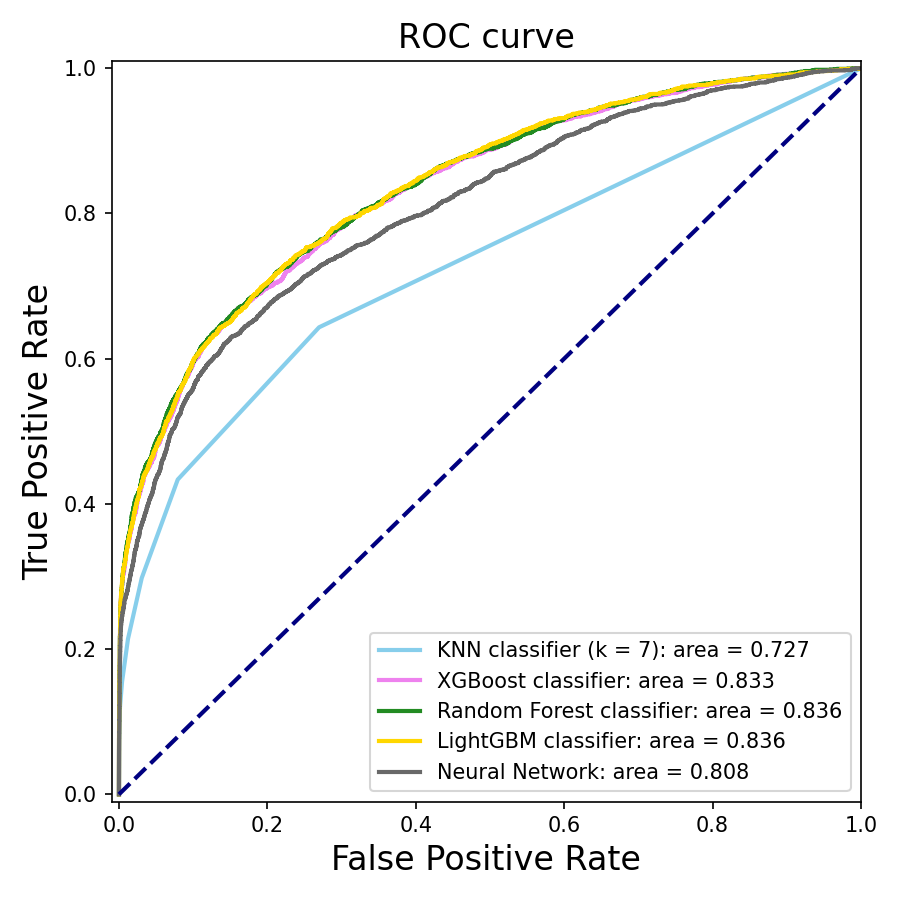
\includegraphics[width=0.7\linewidth,keepaspectratio]{plots/roc_all.png}
\caption{ROC curves of models with optimal hyperparameters on the validation set.}\label{rocplots}
\end{center}
\end{figure}

We see that, within the model hyperparameter spaces we probed, the tree-based classifiers namely \verb|XGBClassifier|, \verb|RandomForestClassifier| and \verb|LGBMClassifier| give the highest auc of $0.833-0.836$. 

For \verb|KNeighborsClassifier|, we got the optimal \verb|k=7|.

For \verb|xgboost.XGBClassifier|, we got the following set of optimal hyperparameters:
\begin{lstlisting}[language=Python, basicstyle=\footnotesize]
XGBC_model = XGBClassifier(scale_pos_weight = (127891.-9247.)/9247., 
                           eval_metric='auc', 
                           n_estimators = 900, 
                           max_depth = 7,
                           learning_rate = 0.01,
                           n_jobs = 8)
\end{lstlisting}
Note that we have addressed class imbalance in training the model using the \verb|scale_pos_weight| of the training set that with which we fit the model.

For \verb|RandomForestClassifier|, we used
\begin{lstlisting}[language=Python, basicstyle=\footnotesize]
RFC = RandomForestClassifier(class_weight = 'balanced', 
                             n_estimators = 700, 
                             max_depth = 20, 
                             max_features= 'auto', 
                             min_samples_leaf = 1, 
                             min_samples_split = 16, 
                             random_state = 0, 
                             n_jobs = -1)
\end{lstlisting}
Here we used \verb|class_weight = 'balanced'|.

For \verb|LGBMClassifier|, 
\begin{lstlisting}[language=Python, basicstyle=\footnotesize]
LGBMclf = lgb.LGBMClassifier(class_weight = 'balanced', 
                             learning_rate = 0.01, 
                            num_leaves = 800,
                            n_estimators = 500, 
                            num_iterations = 900, 
                            max_bin = 500, 
                            feature_fraction = 0.7, 
                            bagging_fraction = 0.7,
                            lambda_l2 = 0.5,
                            max_depth = 7,
                            silent = False)
\end{lstlisting}
and we used \verb|eval_metric = 'auc'| when we fit the model.


\section{Predictions}

Using \verb|LGBMClassifier|, the test set predictions take the following distribution:

\begin{figure}[H]
\centering
\begin{subfigure}{0.6\textwidth}
  \centering
  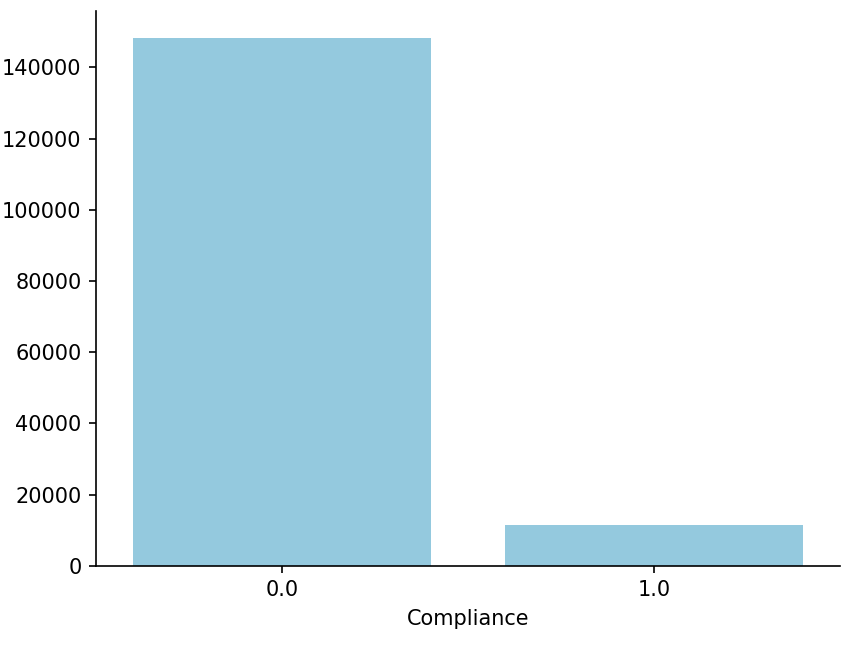
\includegraphics[width=1.\linewidth,keepaspectratio]{plots/train_compliance.png}
\caption{Training set compliance}\label{pred1}
\end{subfigure}% 
\hspace*{-2cm}
\begin{subfigure}{.6\textwidth}
  \centering
  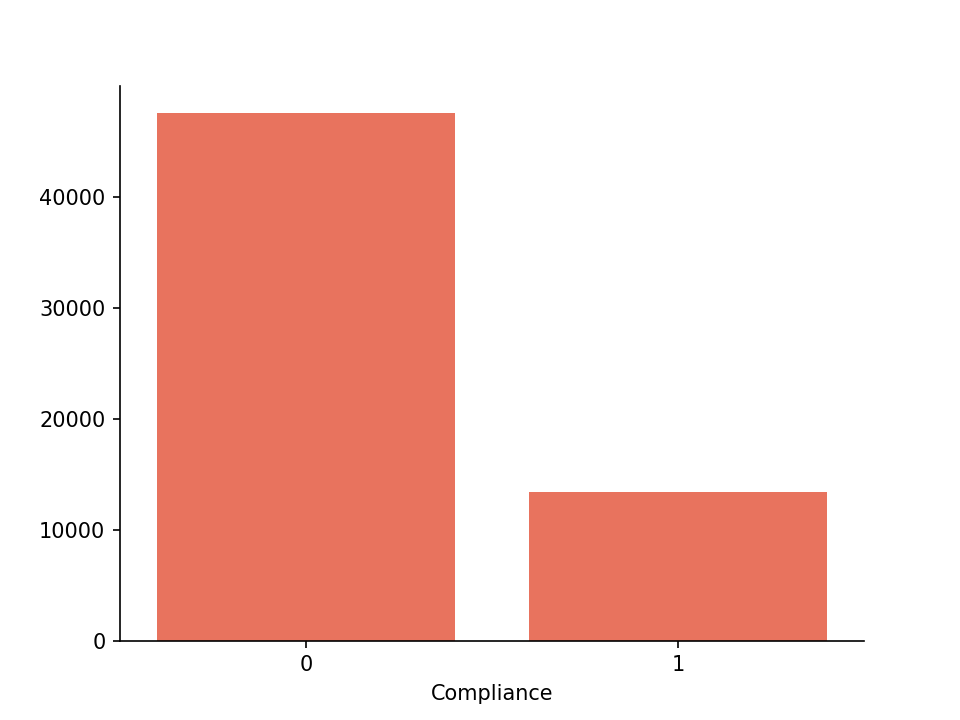
\includegraphics[width=1.\linewidth,keepaspectratio]{plots/test_compliance.png}
  \caption{Test set compliance (predicted)}\label{pred2}
\end{subfigure}
\caption{Compliance: training set VS test set predictions using \texttt{LGBMClassifier}.}
\label{pred}
\end{figure}

Here we have included the training set plot \hyperref[compliance]{Figure \ref*{compliance}} in \hyperref[pred1]{Figure \ref*{pred1}} for comparison. It appears that the predicted test set has a larger proportion of tickets being compliant.

Our original attempt, for the submission of the assignment, achieved slightly lower validation auc's in general. The test auc from the best performing model was $0.774$, which was slight lower than the validation auc's. Possible remedies include regularising the models to reduce overfitting. We expect the current approach to result in a better test auc.

Finally, we look at the feature importances of the best performing models, \verb|XGBClassifier|, \verb|RandomForestClassifier| and \verb|LGBMClassifier|.

\begin{figure}[H]
\begin{center}
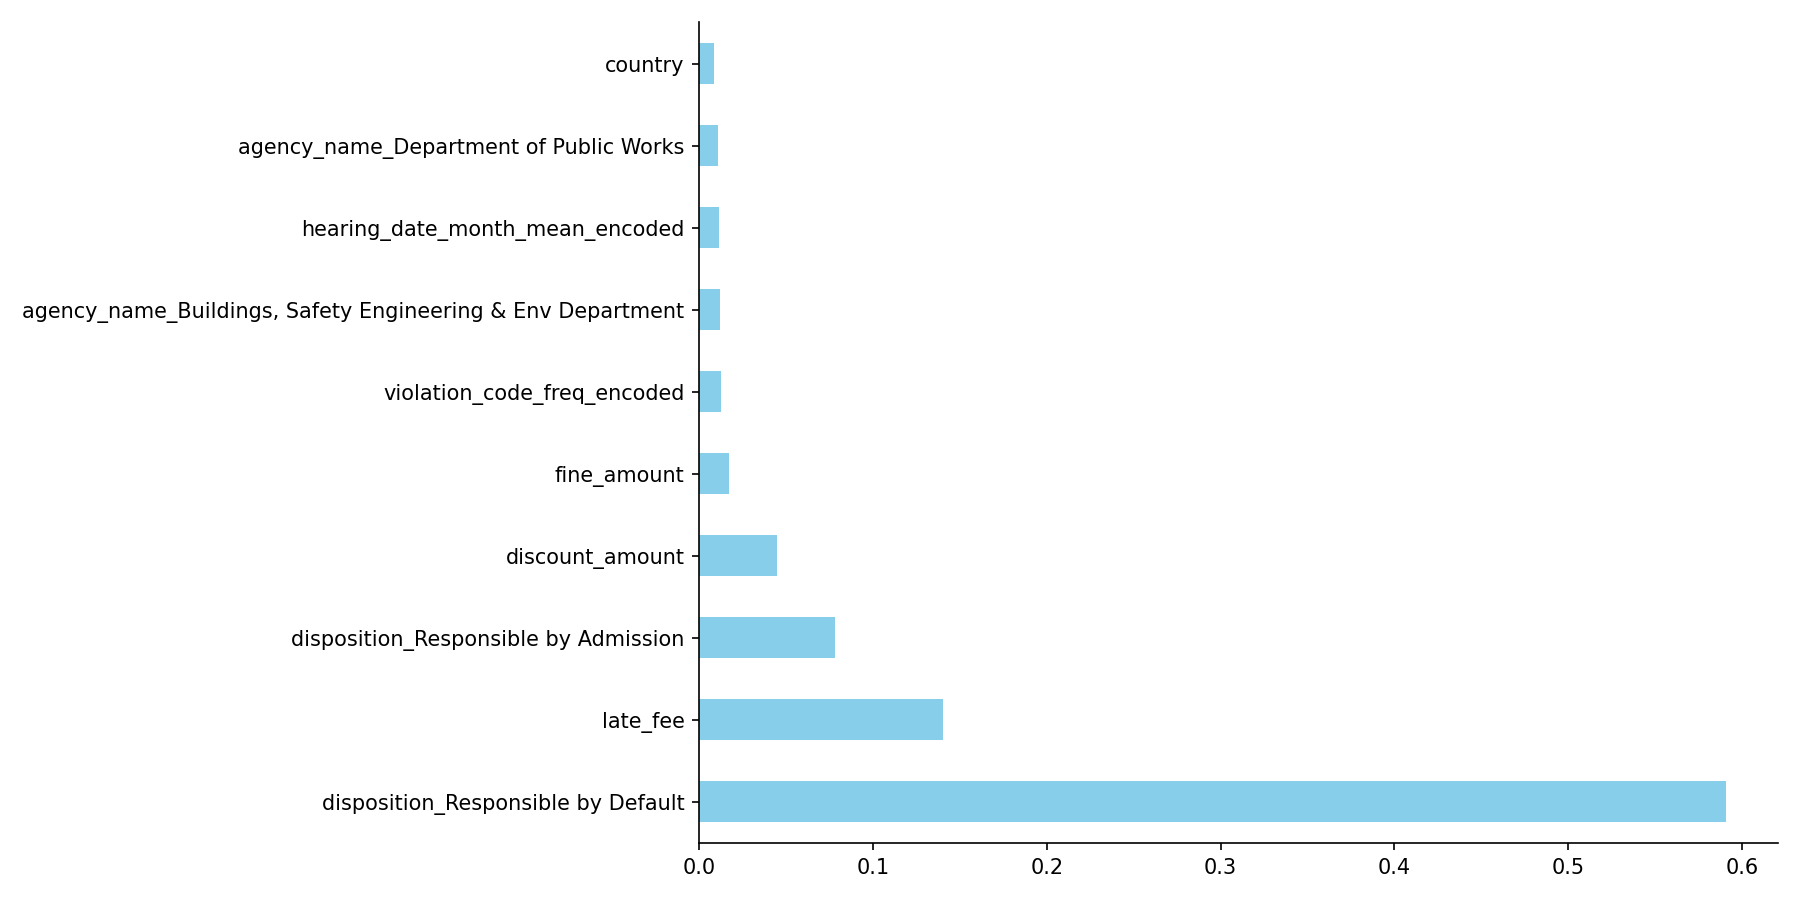
\includegraphics[width=1.\linewidth,keepaspectratio]{plots/XGBM_feature_imp.png}
\caption{Feature importances in \texttt{XGBClassifier}.}\label{xgbmfeat}
\end{center}
\end{figure}

\begin{figure}[H]
\begin{center}
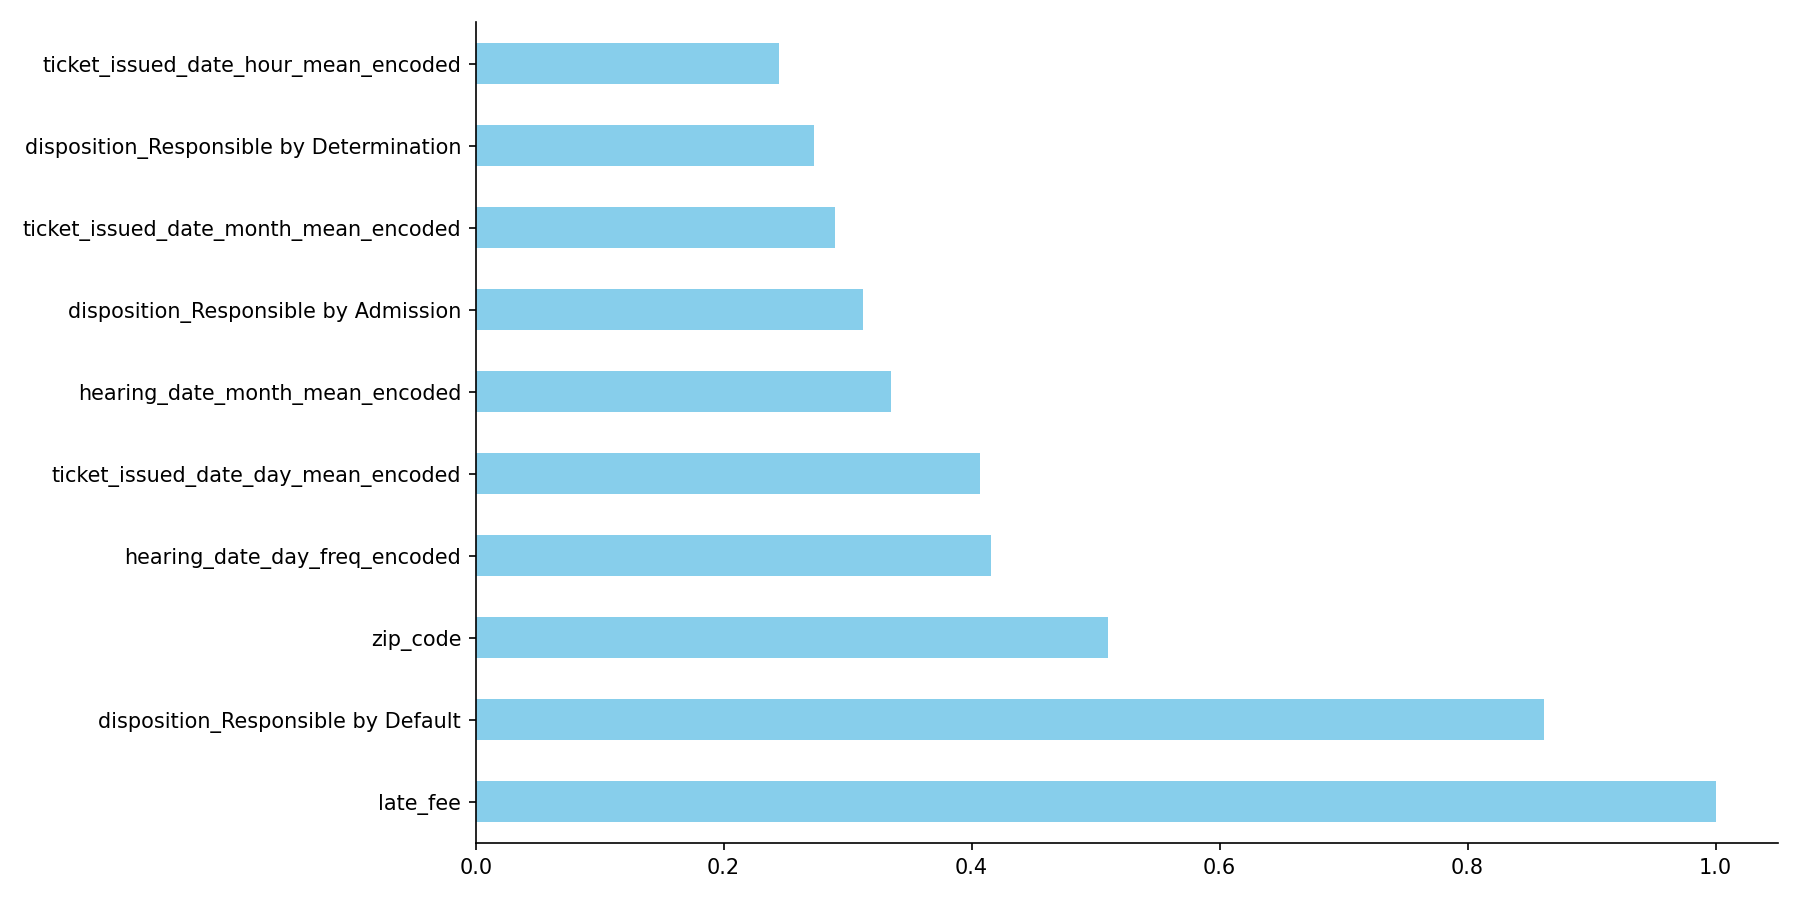
\includegraphics[width=1.\linewidth,keepaspectratio]{plots/RFC_feature_imp.png}
\caption{Feature importances in \texttt{RandomForestClassifier}.}\label{rfcfeat}
\end{center}
\end{figure}

\begin{figure}[H]
\begin{center}
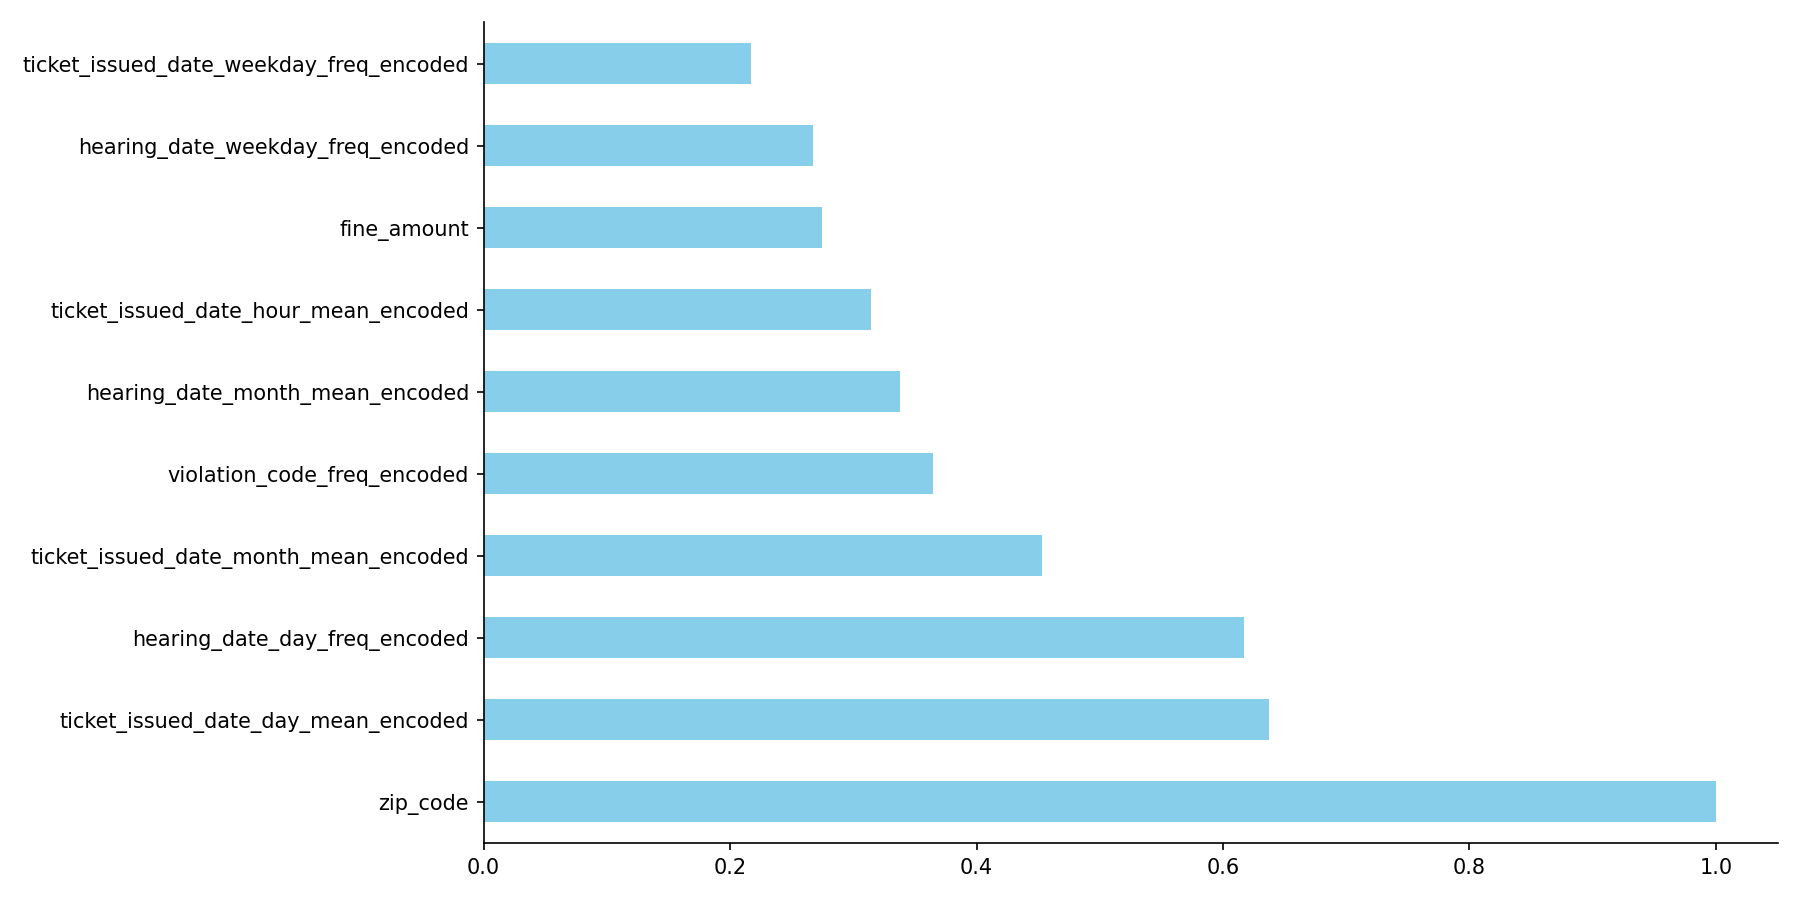
\includegraphics[width=1.\linewidth,keepaspectratio]{plots/LGBM_feature_imp.png}
\caption{Feature importances in \texttt{LGBMClassifier}.}\label{lgbmfeat}
\end{center}
\end{figure}

\vspace*{-12pt}

Though the features importances vary among different models, we can make sense of some of them. For instance, it makes sense that compliance depends on \\\verb|deposition_Responsible by Default|: if the violator does not show up in the hearing, it is natural to expect him/her to not comply with the ticket payment either. It also makes sense that \verb|zip_code| of the mailing address is important; zip codes with lower incomes and higher poverty rates may have lower compliance. 


\section{An Aside}

Out of curiosity, we looked at the mean compliance rate of each month (of the ticket issued date) in the training set; this is a time series. We plotted the auto-correlation and partial auto-correlation:


\begin{figure}[H]
\centering
\begin{subfigure}{0.6\textwidth}
  \centering
  \includegraphics[width=.9\linewidth,keepaspectratio]{plots/1_datetime/ticket_training_acf.png}
\caption{Auto-correlation}\label{acf}
\end{subfigure}% 
\hspace*{-1.5cm}
\begin{subfigure}{.6\textwidth}
  \centering
  \includegraphics[width=.9\linewidth,keepaspectratio]{plots/1_datetime/ticket_training_pacf.png}
  \caption{Partial auto-correlation}\label{pacf}
\end{subfigure}
\caption{Auto-correlation and partial auto-correlation of monthly mean compliance in the training set.}
\label{acfpacf}
\end{figure}

We see that the auto-correlation decays gradually from zero lag, while the partial auto-correlation is large at lag=one month only. We conclude that it appears to be described by an auto-regressive AR(1) model.


\section{Acknowledgment}

We acknowledge the authors from various sources online, whose tools and techniques were borrowed and implemented in our codes. (I didn't keep track of the references.)


%
%\renewcommand\refname{References}
%\bibliographystyle{utphys}
%\bibliography{references}
%
%\begin{filecontents}[overwrite]{references.bib}
%@article{Dymarsky:2020qom,
%    author = "Dymarsky, Anatoly and Shapere, Alfred",
%    title = "{Quantum stabilizer codes, lattices, and CFTs}",
%    eprint = "2009.01244",
%    archivePrefix = "arXiv",
%    primaryClass = "hep-th",
%    doi = "10.1007/JHEP03(2021)160",
%    journal = "JHEP",
%    volume = "21",
%    pages = "160",
%    year = "2020"
%}
%
%@book{Zwillinger,
%  author    = {Zwillinger, D.}, 
%  title     = {Standard Mathematical Tables and Formulae},
%  publisher = {Academic Press},
%  year      = 2003,
%  edition   = 8,
%  isbn      = {978-0-12-384933-5}
%}
%
%
%\end{filecontents}


\end{document}

